% begin module continuous-def
\begin{frame}
\frametitle{Continuity}
\begin{definition}[Continuous at a Number]
A function $f$ is continuous at a number $a$ if
\[
\lim_{x\rightarrow a}f(x) = f(a) .
\]
\end{definition}
\begin{columns}[c]
\column{.5\textwidth}
\psset{xunit=1cm, yunit=1cm}
\begin{pspicture}(-1, -0.5)(4,3.5) \psframe*[linecolor=white](-1,-0.5)(4,3.5) \psaxes[labels=none]{<->}(0,0)(-0.5,-0.5)(4,3)
\psplot[linecolor=red, plotpoints=1000]{-0.5}{4}{x 0.5 mul 4 exp 0.125 mul x 0.5 mul 2 exp -1 mul add x 0.5 mul 3 exp 0.5 mul add 1 add }
\end{pspicture} 
%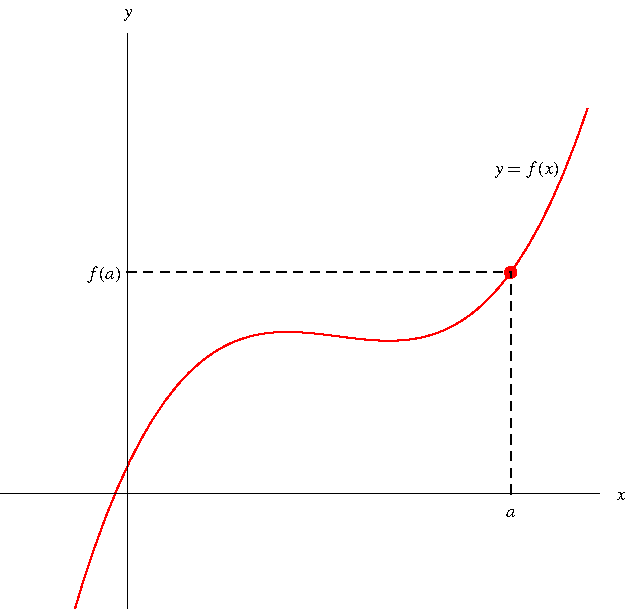
\includegraphics[height=4.5cm]{continuity/pictures/02-05-continuous.pdf}%
\column{.5\textwidth}
\uncover<2->{
The definition (implicitly) requires the following.
\begin{enumerate}
\item  $f(a)$ is defined (i.e., $a$ is in the domain of $f$).
\item  $\lim\limits_{x\rightarrow a}f(x)$ exists.
\end{enumerate}
}
\end{columns}
\end{frame}
% end module continuous-def

